\documentclass{article}
\usepackage{graphics,hyperref,amsmath,amsfonts}
\usepackage{lscape}
\begin{document}
\title{An Introduction to Information Retrieval, Part II}
\author{STA 325}
\date{October 5, 2018}
\maketitle

\begin{center}
  \textsc{Reading}: {\em Principles of Data Mining}, sections\ 14.1--14.4
  (skiping 14.3.3 for now) and 3.7.
\end{center}

Let's recap where we left similarity searching for documents.  We represent
each document as a {\bf bag of words}, i.e., a vector giving the number of
times each word occurred in the document.  This abstracts away all the
grammatical structure, context, etc., leaving us with a matrix whose rows are
feature vectors, a data frame.  To find documents which are similar to a given
document $Q$, we calculate the distance between $Q$ and all the other
documents, i.e., the distance between their feature vectors.

\section{Queries}

If we have a document in hand which we like, and we want to find the $k$
documents closest to it, we can do this once we know the distances between that
document and all the others.  But how can we get away from finding that
one good document to begin with?

The trick is that a query, whether an actual sentence (``What are the common
problems of the 2001 model year Saturn?'') or just a list of key words
(``problems 2001 model Saturn'') {\em is} a small document.  If we represent
user queries as bags of words, we can use our similarity searching procedure on
them.  This is really all it takes.

%\subsection{Evaluating Similarity Search}
%
%When someone uses a search engine, they have some idea of which of the results
%are what they were looking for.  In the jargon, we say that the good results
%were {\bf relevant} to the query.  There are actually two aspects to
%finding relevant documents, both of which are important:
%\begin{itemize}
%\item Most of the results should be relevant; that is, the {\bf precision} of
%  the search should be high.
%\item Most of the relevant items should be returned as results; that is, the
%  {\bf recall} should be high, too.
%\end{itemize}
%
%Formally, if the search returns $k$ items, $r$ of which are relevant, and there
%are $R$ relevant items in the whole corpus of $N$ items, the precision is the
%ratio $r/k$, and the recall is the ratio $r/R$.  (This is for one query, but we
%can average over queries.)  Notice that $r \leq k$, so there are limits on how
%high the recall can be when $k$ is small.  As we change $k$ for a given query,
%we get different values for the precision and the recall.  Generally, we expect
%that increasing $k$ will increase recall (more relevant things can come in) but
%lower precision (more irrelevant things can come in, too).  A good search
%method is one where the trade-off between precision and recall is not very
%sharp, where we can gain a lot of recall while losing on a little precision.
%
%A visual way of representing the precision-recall trade-off is to plot
%precision (on the vertical axis) against recall (on the horizontal axis) for
%multiple values of $k$.  If the method is working well, when $k$ is small the
%precision should be high, though the recall will be limited by $k$; as $k$
%grows, the recall should increase, moving us to the right, but the recall will
%fall, moving us down.  So the precision-recall curve should going from
%somewhere near $(1,0)$ to somewhere near $(0,1)$.  The total {\bf area under
%  the curve} is often used as a measure of how good the search method is.
%
%Of course, there is nothing magic about changing $k$; if we have a different
%search technique with a tunable setting, we can make a precision-recall curve
%for it, too.
%
%\paragraph{Search, Hypothesis Testing, Signal Detection, ROC} It is no
%coincidence that the difference between precision and recall is very like the
%difference between type I and type II errors in hypothesis testing.  High
%precision is like having a low type I error rate (most of the ``hits' are
%real); high recall is like having a low type II error rate (most things which
%should be hits are).
%
%The same idea applies to {\bf signal detection} as well, where a type I error
%is called a ``false alarm'' (you thought there was signal when there was just
%noise) and a type II error is called a ``miss'' (you mistook signal for noise).
%The precision-recall curves actually come from signal detection theory, where
%they are called {\bf receiver operating characteristic} curves, or {\bf ROC}
%curves.
%
%\paragraph{Practice} In practice, the only way to tell whether your
%search-engine's results are relevant is to ask actual people (Figure
%\ref{fig:relevant}).  The major services do this with lab experiments, with
%special browsers given to testers to ask quiz them on whether the results were
%relevant, and by taking random samples of their query log and having testers
%repeat the queries to see whether the results were relevant.  Naturally, this
%use of human beings is slow and expensive, especially because the raters have
%to be trained, so the amount of this data is limited --- and they are {\em
%  very} reluctant to share it.
%
%
%Notice, by the way, that when dealing with something like the web, or indeed
%any large collection where users give arbitrary queries, it is a lot easier to
%estimate precision than recall (how do you find $R$, the number of genuinely
%relevant documents in the whole corpus?).
%
%
%\section{Classification}
%
%One very important data-mining task is {\bf classifying} new pieces of data,
%that is, assigning them to one of a fixed number of {\bf classes}.  Last time,
%our two classes were ``stories about music'' and ``stories about the other
%arts''.  Usually, new data doesn't come with a class label, so we have to
%somehow guess the class from the features.\footnote{If it does come with a
%  label, we read the label.}  Two very basic strategies become available
%as soon as we can measure similarity or distance.
%\begin{enumerate}
%\item With a {\bf nearest neighbor} strategy, we guess that the new object is
%  in the same class as the closest already-classified object.  (We saw this at
%  the end of the last lecture.)  Similarity search is in a way just the
%  reverse: we guess that the nearest neighbor is in the same class (``is
%  relevant'') as the query.
%\item With a {\bf prototype} strategy, we pick out the ``most representative''
%  member of each class, or perhaps the average of each class, as its prototype,
%  and guess that new objects belong to the class with the closer prototype.
%\end{enumerate}
%We will see many other classification methods before the course is over.
%
%All classification methods can be evaluated on their {\bf error rate} or {\bf
%  mis-classification rate}, which is simply the fraction of cases they get
%wrong, by assigning them to the wrong class.  (A classifier's
%mis-classification rate is also sometimes just called its {\bf inaccuracy}.)  A
%more refined analysis distinguishes between different kinds of errors.  For
%each class $i$, we record what fraction of $i$'s are guessed to be of class
%$j$, and get a little matrix called the {\bf confusion matrix}.  (The diagonal
%entries show probabilities of correct classifications.)  For two classes, this
%gives us the type I and type II error rates again --- though which is which is
%arbitrary.

\section{Inverse Document Frequency}

Someone asked in class last time about selectively paying less attention to
certain words, especially common words, and more to the rest.  This is an
excellent notion.  Not all features are going to be equally useful, and some
words are so common that they give us almost no ability at all to discriminate
between relevant and irrelevant documents.  In (most) collections of English
documents, looking at ``the'', ``of'', ``a'', etc., is a waste of time.  We
could handle this by a fixed list of {\bf stop words}, which we just don't
count, but this at once too crude (all or nothing) and too much work (we need
to think up the list).

{\bf Inverse document frequency} (IDF) is a more adaptive approach.  The {\bf
  document frequency} of a $w$ is the number of documents it appears in, $n_w$.
The IDF weight of $w$ is 
\[
IDF(w) \equiv \log{\frac{N}{n_w}}
\]
where $N$ is the total size of our collection.  Now when we make our
bag-of-words vector for the document $Q$, the number of times $w$ appears in
$Q$, $Q_w$, is multiplied by $IDF(w)$.  Notice that if $w$ appears in every
document, $n_w = N$ and it gets an IDF weight of zero; we won't use it to
calculate distances.  This takes care of most of the things we'd use a list of
stop-words for, but it also takes into account, implicitly, the kind of
documents we're using.  (In a data base of papers on genetics, ``gene'' and
``DNA'' are going to have IDF weights of near zero too.)  On the other hand, if
$w$ appears in only a few documents, it will get a weight of about $\log{N}$,
and all documents containing $w$ will tend to be close to each other.


Table \ref{table:idf-is-good} shows how including IDF weighting, along with
Euclidean length normalization, dramatically improves our ability to classify
posts as either about music or about the other arts.

\begin{table}
  \begin{center}
    \begin{tabular}{ccc}
      Normalization & Equal weight & IDF weight \\
      \hline
      None             & 38 & 52 \\
      Word count  & 39 & 37 \\
      Euclidean length & 44 & 19 \\
    \end{tabular}
    \caption{Number of mis-classifications in a collection of 102 stories from
      the {\em Times} about music (45 stories) and the other arts (57 stories)
      when using the nearest neighbor method, with different choices of
      normalization and with or without IDF weighting.  (Cf.\ Fig.\
      \ref{fig:mds}.)  Note that an idiot who always guessed ``art'' would only
      make 45 mistakes.}
    \label{table:idf-is-good}
  \end{center}
\end{table}

You could tell a similar story about any increasing function, not just $\log$,
but $\log$ happens to work very well in practice, in part because it's not very
sensitive to the exact number of documents.  So this is not the same $\log$ we
will see in information theory, or the $\log$ in psychophysics.  Notice also
that this is {\em not} guaranteed to work.  Even if $w$ appears in every
document, so $IDF(w) = 0$, it might be common in some of them and rare in
others, so we'll ignore what might have been useful information.  (Maybe
genetics papers about laboratory procedures use ``DNA'' more often, and papers
about hereditary diseases use ``gene'' more often.)

--- This is our first look at the problem of {\bf feature selection}: how do we
pick out good, useful features from the very large, perhaps infinite,
collection of possible features?  We will come back to this in various ways
throughout the course.  Right now, concentrate on the fact that in search,
and other classification problems, we are looking for features that let us
{\bf discriminate} between the classes.



\section{More Wrinkles to Similarity Search}

\subsection{Stemming}

It is a lot easier to decide what counts as ``a word'' in English than in some
other languages.\footnote{For example, Turkish is what is known as an
  ``aggulutinative'' language, in which grammatical units are ``glued
  together'' to form compound words whose meaning would be a whole phrase or
  sentence in English, e.g., {\em gelemiyebelirim}, ``I may be unable to
  come'', {\em yapabilecekdiyseniz}, ``if you were going to be able to do'', or
  {\em calistirilmamaliymis}, ``supposedly he ought not to be made to work''.
  (German does this too, but not so much.)  This causes problems with
  Turkish-language applications, because many
  sequences-of-letters-separated-by-punctuation are effectively unique.  See,
  for example, L. {\"O}zg{\"u}r, T. G{\"u}ng{\"o}r and F. G{\"u}rgen,
  ``Adaptive anti-spam filtering for agglutinative languages: a special case
  for Turkish'', {\em Pattern Recognition Letters} {\bf 25} (2004): 1819--1831,
  available from \url{http://www.cmpe.boun.edu.tr/~gungort/}.}  Even so, we
need to decide whether ``car'' and ``cars'' are the same word, for our
purposes, or not.  {\bf Stemming} takes derived forms of words (like ``cars'',
``flying'') and reduces them to their stem (``car'', ``fly'').  Doing this well
requires linguistic knowledge (so the system doesn't think the stem of
``potatoes'' is ``potatoe'', or that ``gravity'' is the same as ``grave''), and
it can even be harmful (if the document has ``Saturns'', plural, it's most
likely about the cars).

\subsection{Feedback}

People are much better at telling whether you've found what they're looking for
than they are at {\em explaining} what it is that they're looking for.  (They
know it when they see it.)  Queries are users trying to explain what they're
looking for (to a computer, no less), so they're often pretty bad.  An
important idea in data mining is that people should do things at which they are
better than computers and vice versa: here they should be deciders, not
explainers.  {\bf Rocchio's algorithm} takes feedback from the user, about
which documents were relevant, and then refines the search, giving more weight
to what they like, and less to what they don't like.

The user gives the system some query, whose bag-of-words vector is $Q_t$.  The
system responses with various documents, some of which the user marks as
relevant ($R$) and others as not-relevant ($NR$).  (See Fig.\
\ref{fig:relevant} again.)  The system then modifies the query vector:
\[
Q_{t+1} = \alpha Q_t + \frac{\beta}{|R|}\sum_{\mathrm{doc} \in R}{\mathrm{doc}} - \frac{\gamma}{|NR|}\sum_{\mathrm{doc}\in NR}{\mathrm{doc}}
\]
where $|R|$ and $|NR|$ are the number of relevant and non-relevant documents,
and $\alpha$, $\beta$ and $\gamma$ are positive constants.  $\alpha$ says how
much continuity there is between the old search and the new one; $\beta$ and
$\gamma$ gauge our preference for recall (we find more relevant items) versus
precision (more of what we find is relevant).  The system then runs another
search with $Q_{t+1}$, and cycle starts over.  As this repeats, $Q_t$ gets
closer to the bag-of-words vector which best represents what the user has in
mind, assuming they have something definite and consistent in mind.

N.B.: A word can't appear in a document a negative number of times, so
ordinarily bag-of-words vectors have non-negative components.  $Q_t$, however,
can easily come to have negative components, indicating the words whose {\em
  presence} is evidence that the document isn't relevant.  Recalling the
example of problems with used 2001 Saturns, we probably don't want anything
which contains ``Titan'' or ``Rhea'', since it's either about mythology or
astronomy, and giving our query negative components for those words suppresses
those documents.

Rocchio's algorithm works with any kind of similarity-based search, not just
text.  It's related to many machine-learning procedures which incrementally
adjust in the direction of what has worked and away from what has not --- the
{\bf stochastic approximation} algorithm for estimating functions and curves,
{\bf reinforcement learning} for making decisions, {\bf Bayesian learning} for
updating conditional probabilities, and {\bf multiplicative weight training}
for combining predictors.  This is no
accident; they are all special cases of adaptive evolution by means of natural
selection.


\section{Visualization: Multidimensional Scaling}

The bag-of-words vectors representing our documents generally live in spaces
with lots of dimensions, certainly more than three, which are hard for ordinary
humans to visualize.  However, we can compute the distance between any two
vectors, so we know how far apart they are.  {\bf Multidimensional scaling}
(MDS) is the general name for a family of algorithms which take
high-dimensional vectors and map them down to two- or three-dimensional
vectors, trying to preserve all the relevant distances.

Abstractly, the idea is that we start with vectors $v_1, v_2, \ldots v_n$ in a
$p$-dimensional space, where $p$ is large, and we want to find new vectors
$x_1, x_2, \ldots x_n$ in $\mathbb{R}^2$ or $\mathbb{R}^3$ such that
\[
\sum_{i=1}^{n}{\sum_{j\neq i}{{\left(\delta(v_1, v_2) - d(x_1,x_2)\right)}^2}}
\]
is as small as possible, where $\delta$ is distance in the original space and
$d$ is Euclidean distance in the new space.  Note that the new or {\bf image}
points $x_i$ are {\em representations} of the $v_i$, i.e., representations of
representations.

There is some trickiness to properly minimizing this \textbf{objective
  function} --- for instance, if we rotate all the $x_i$ through a common
angle, their distances are unchanged, but it's not really a new solution ---
and it's not usually possible to make it exactly zero (See Sec.\ 3.7 in the
textbook for details.)  We will see a lot of multidimensional scaling plots,
because they are nice visualization tools, but we will also see a lot of other
{\bf data reduction} or {\bf dimensionality reduction} methods, because
sometimes it's more important to preserve {\em other} properties than
distances.

Notice that while the bag of words representation gives each of our original
coordinates/features some meaning --- it says something very definite about the
document being represented --- that's not the case with the coordinates we get
after doing the MDS.  If nothing else, the fact that we could rotate all of the
image points arbitrarily makes it very hard to assign any interpretation to
where the images fall on the axes.  This is true of many other
dimensionality-reduction methods as well.

\begin{figure}
\begin{center}
\resizebox{0.65\textwidth}{!}{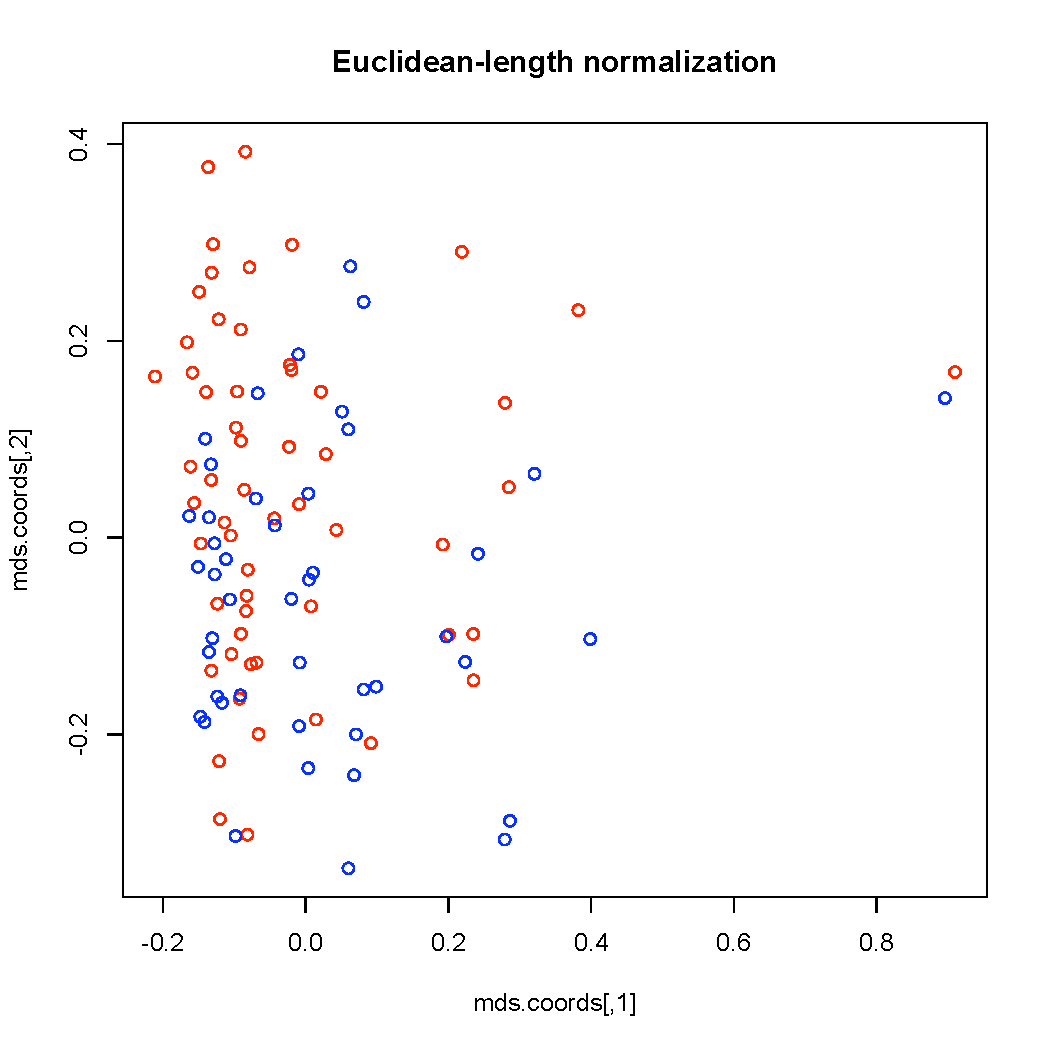
\includegraphics{mds_euc_no_idf}}
\resizebox{0.65\textwidth}{!}{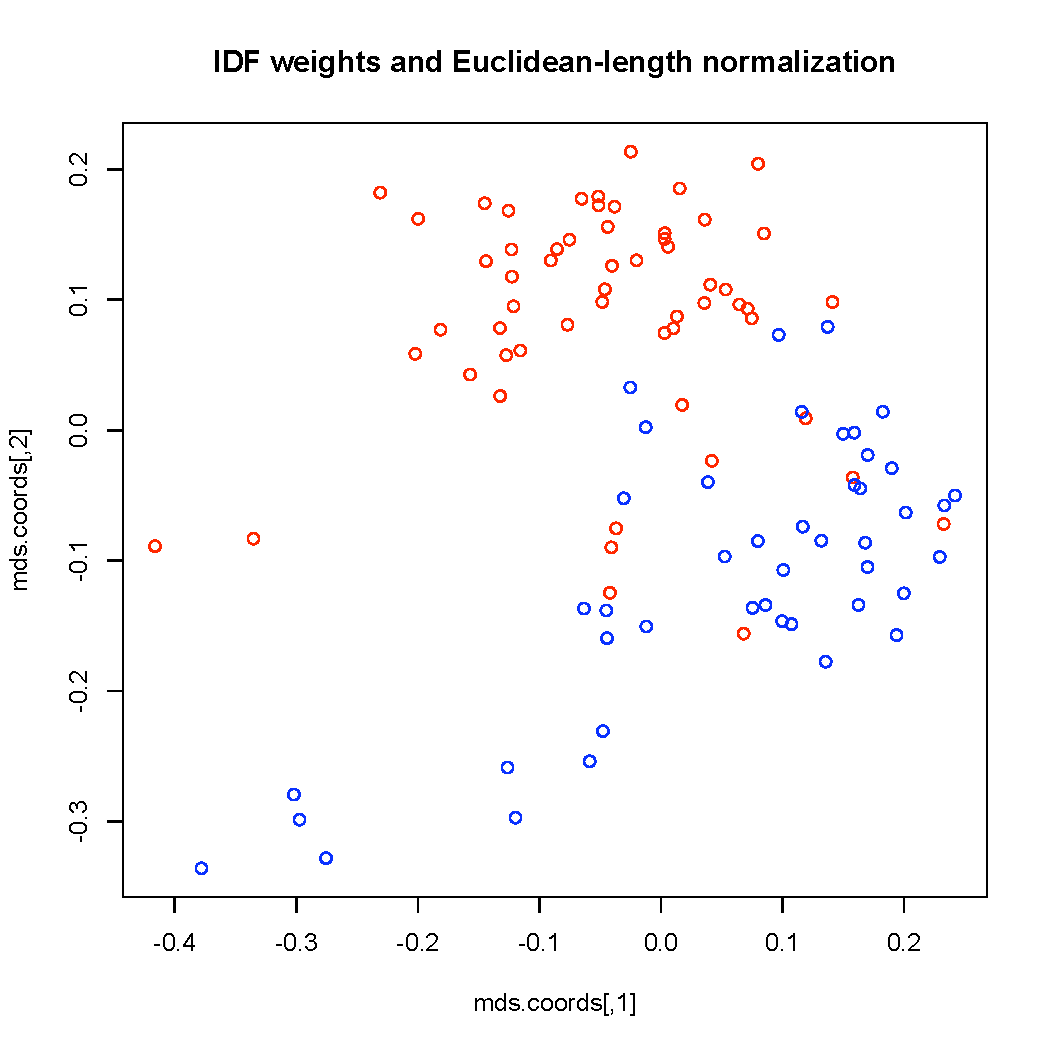
\includegraphics{mds_euc_idf}}
\end{center}
\caption{Illustrations of multidimensional scaling for the 102 art/music
  stories (art=red, music=blue), with and without IDF weights.  This was
  produced using the R command \texttt{cmdscale} (plus a little extra code to
  plot it nicely).  Notice that with IDF weights, the two classes are far more
  distinct visually, which comes through in the classification results in Table
  \ref{table:idf-is-good}.}
\label{fig:mds}
\end{figure}
\end{document}
